%%%%%
%%Title: HiPi+Bus V0.2 Chapter 8
%%Creator: Ando Ki
%%CreationDate: April 1992
%%FileName: sec1
%%RelatedFile: ch8
%%%%%
\section{개요}
버스의 기계적 규격은 백플레인(backplane), 백플레인에 꽂혀 사용될 보드(board),
백플레인과 보드를 지지하는 서브랙(subrack),
%각 보드간의 전달신호를 안정되게 하는 터미네이터(terminator),
% 보드에 공급될 버스클럭을 공급하는 버스클럭,
각 보드에서 필요로 하는 주전원 전력을 균등하게 공급하도록 하는 파워 바(power bar),
%주전원 이외의 전원 공급을 위한 파워 탭(power tab),
그리고 백플레인과 보드를 연결하는 콘넥터의 규격을 정의한다.
%
\begin{figure}[htb]
    \centerline{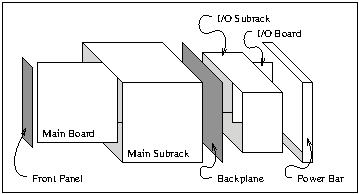
\includegraphics{ch8/FIG/mech-over.jpg}}
   \caption{기계적 장치의 개요}\label{figure:mech-over}
\end{figure}
%
\begin{itemize}
  \item front panel (전면판넬) : HiPi+Bus main board의 전면에 설치되는 전면 판넬이다.
  \item main board (주보드) : HiPi+Bus 백플레인에 꽂히게 될 보드이다.
  \item main subrack (주서브랙) : main board가 백플레인의 슬롯에 꽂힐때 제대로 꽂히도록 지지하는 기구물이다.
  \item backplane (백플레인) : HiPi+Bus 백플레인이다.
  \item I/O subrack (입출력서브랙) : I/O board가 백플레인의 뒷쪽 슬롯에 꽂힐때 제대로 꽂히도록 지지하는 기구물이다.
  \item I/O board (입출력보드) : HiPi+Bus 백플레인 뒷쪽 슬롯에 꽂히게 될 보드로 I/O bus와의 연결을
		용이하게 하기 위한 보드이다.
  \item power bar (파워바) : HiPi+Bus 백플레인의 뒷쪽에 설치되어 백플레인을 통해 백플레인에 꽂히는 모든 보드에
		전원을 공급하고 분배하는 장치이다.
\end{itemize}
%%%%%
